\begin{usecase}{Logout}
  \ucbasicinfo{High}{Regular}
  \ucshortdescription{This UC allows the user to logout from the app.}
  \uctrigger{This UC is triggered when logout button in the settings page is clicked.}
  \ucactors{User}{None}
  \ucpreconditions{The user must be logged in.}
  \ucrelationships{N/A}{N/A}{N/A}
  \ucmainflow{
    \begin{enumerate}
      \item The user click the logout button
            \ucinfo{The app deletes the JWT and moves the user to the onboarding screen.}
    \end{enumerate}
  }
  \ucconclusion{The user is logged out.}
  \ucpostconditions{The user will be logged out from the system}
\end{usecase}

\begin{figure}[!h]
  \centering
  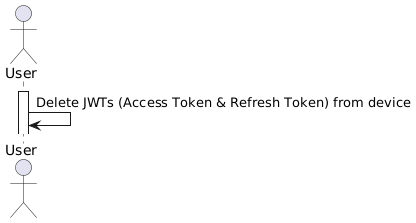
\includegraphics[width=0.3\textwidth]{images/docs/diagrams/sequence-diagrams/all-sequence-diagrams/Logout.png}
  \caption{Logout Sequence Diagram}
  \label{fig:seq/logout}
\end{figure}

The ``Logout Sequence Diagram'', shown in \textbf{Figure~\ref{fig:seq/logout}}, demonstrates the secure logout process in Jadwal. Unlike other operations that require server interaction, the logout process is handled entirely on the client side for efficiency and immediate security effect. When the user initiates logout, the application immediately removes the JWT (JSON Web Token) from the device's secure storage.

This local-only operation ensures immediate session termination, as any subsequent requests would fail without the authentication token. This approach provides several benefits:
\begin{itemize}
  \item Instant logout response, regardless of network conditions
  \item Guaranteed security even if network connectivity is lost
  \item Clean session termination without server-side state management
\end{itemize}

After token removal, the user is automatically redirected to the onboarding screen, effectively preventing any further access to authenticated features until a new login is performed.